% done
\part{Support Vector Classifier}
\label{part:svc}

%------------------------------------

\section{About this part}
\label{section:SVC_about_part}

Now that a fine-tuned linear baseline model is established, the search for better models can start.
Sci Kit learn has a flow chart for deciding which estimator to use, \href{https://scikit-learn.org/stable/tutorial/machine_learning_map/index.html}{available here}.
When following this chart a Support Vector Classifier (SVC) is proposed, thus one is examined here.
Since part \ref{part:linear_baseline} already exhaustively discusses the model testing strategy used, this part will go into less detail to avoid repetition. 
The Notebook corresponding with this part is \texttt{support\_vector\_classifier.ipynb}.


%------------------------------------

\section{Scoring and methodology for fine-tuning}
\label{section:SVC_methodology}

Again, the multi-class Log Loss (MCLL) score is used to compare models.
\texttt{GridSearchCV} was used to find optimal parameters were no human reasoning is needed.
Figure \ref{fig:3-clusters} shows the results of experimenting with different clusters and descriptors.
It is noted that overfitting is clearly visible when using over 250 clusters.
For the final model SIFT with 100 clusters is used.

Balancing the class weight had a small positive impact, which is great!
The non-balanced one is discussed here but found parameters and reasoning are identical for both.
Making the toll more precise had a negligible impact (-0.00) on the results thus it is left default.
\texttt{GridSearchCV} was used to find the optima for C and gamma for the \textit{rbf}, \textit{sigmoid} and \textit{poly} kernel.
For the poly kernel, it was also used to find an optimal degree.
It was insured \texttt{GridSearchCV} uses Stratified K-Folds cross-validation (SCV) with MCLL scoring to keep the unbalance of classes in mind.
What follows are tested parameters and the found optimal for each of these experiments:
\begin{itemize}
    \item Rbf kernel
    \begin{itemize}
        \item Tested C: 0.001, 0.01 , 0.1, 0.5, 1.0, 1.5, 3, 5, 10 and 100.
        \item Tested gamma: "scale", "auto", 0.001, 0.01 , 0.1, 0.5, 1.0, 1.5, 3, 5, 10 and 100.
        \item Found optima: C = 1.5 | gamma = 0.01, auto or scale | SCV MCLL score of ± 1.46.
    \end{itemize}
    \item Sigmoid kernel
    \begin{itemize}
        \item Tested C: 0.001, 0.01 , 0.1, 0.5, 1.0, 1.5, 3, 5, 10 and 100.
        \item Tested gamma: "scale", "auto", 0.001, 0.01 , 0.1, 0.5, 1.0, 1.5, 3, 5, 10 and 100.
        \item Found optima: C = 5 or 10 | gamma = 0.001 | SCV MCLL score of ± 1.54.
    \end{itemize}
    \item Poly kernel:
    \begin{itemize}
        \item Tested C: 0.1, 0.5, 1.0, 1.5, 3 and 5.
        \item Tested gamma: "scale", "auto", 0.001, 0.01 , 0.1, 0.5, 1.0 and 1.5.
        \item Tested degree: 2, 3, 4, 5, 7 and 10.
        \item Found optima: C between 1 and 5 | degree = 3 | gamma = scale, auto or 0.01  | SCV MCLL score of ± 1.59.
    \end{itemize}
\end{itemize}

\begin{figure*}[ht]
    \centering
    \begin{subfigure}{.45\textwidth}
        \centering
        \fbox{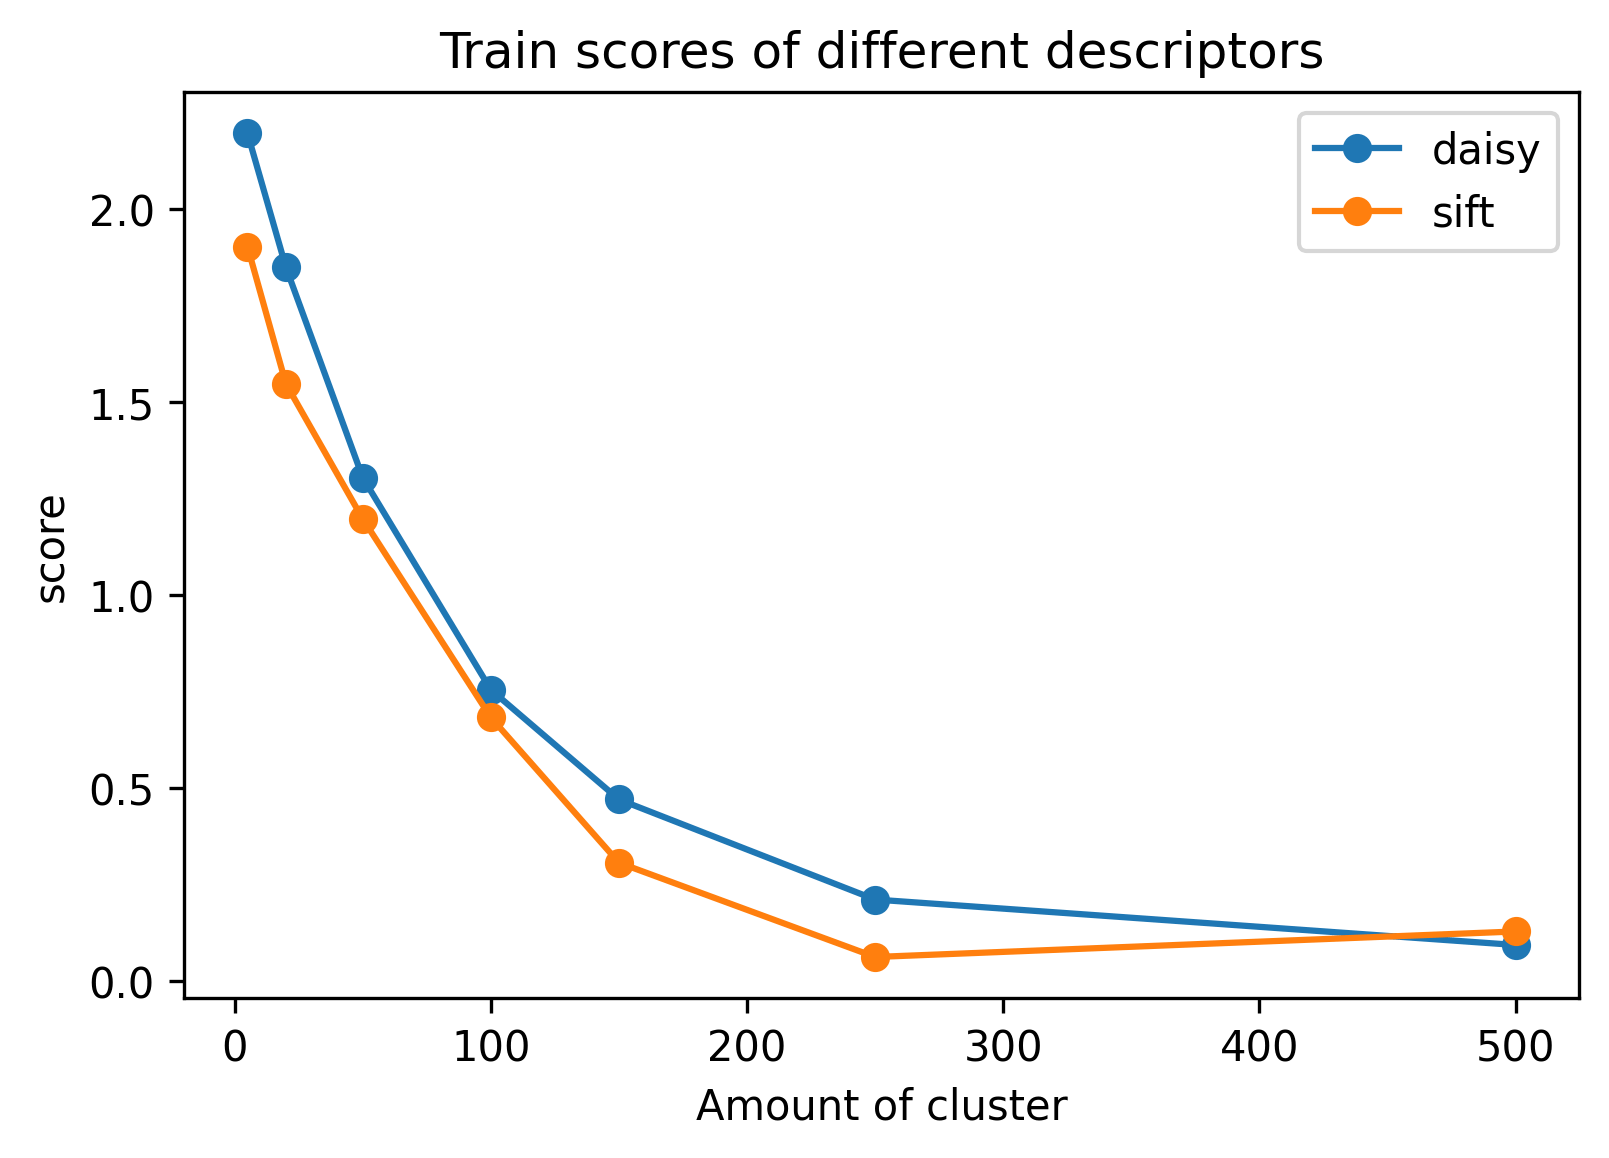
\includegraphics[width=\textwidth]{images/3/3_different_descriptors_train.png}}
        \captionsetup{width=0.9\linewidth}
        \captionsetup{justification=centering}
        \caption{Train scores.}
    \end{subfigure}
    \hspace{1cm}
    \begin{subfigure}{.45\textwidth}
        \centering
        \fbox{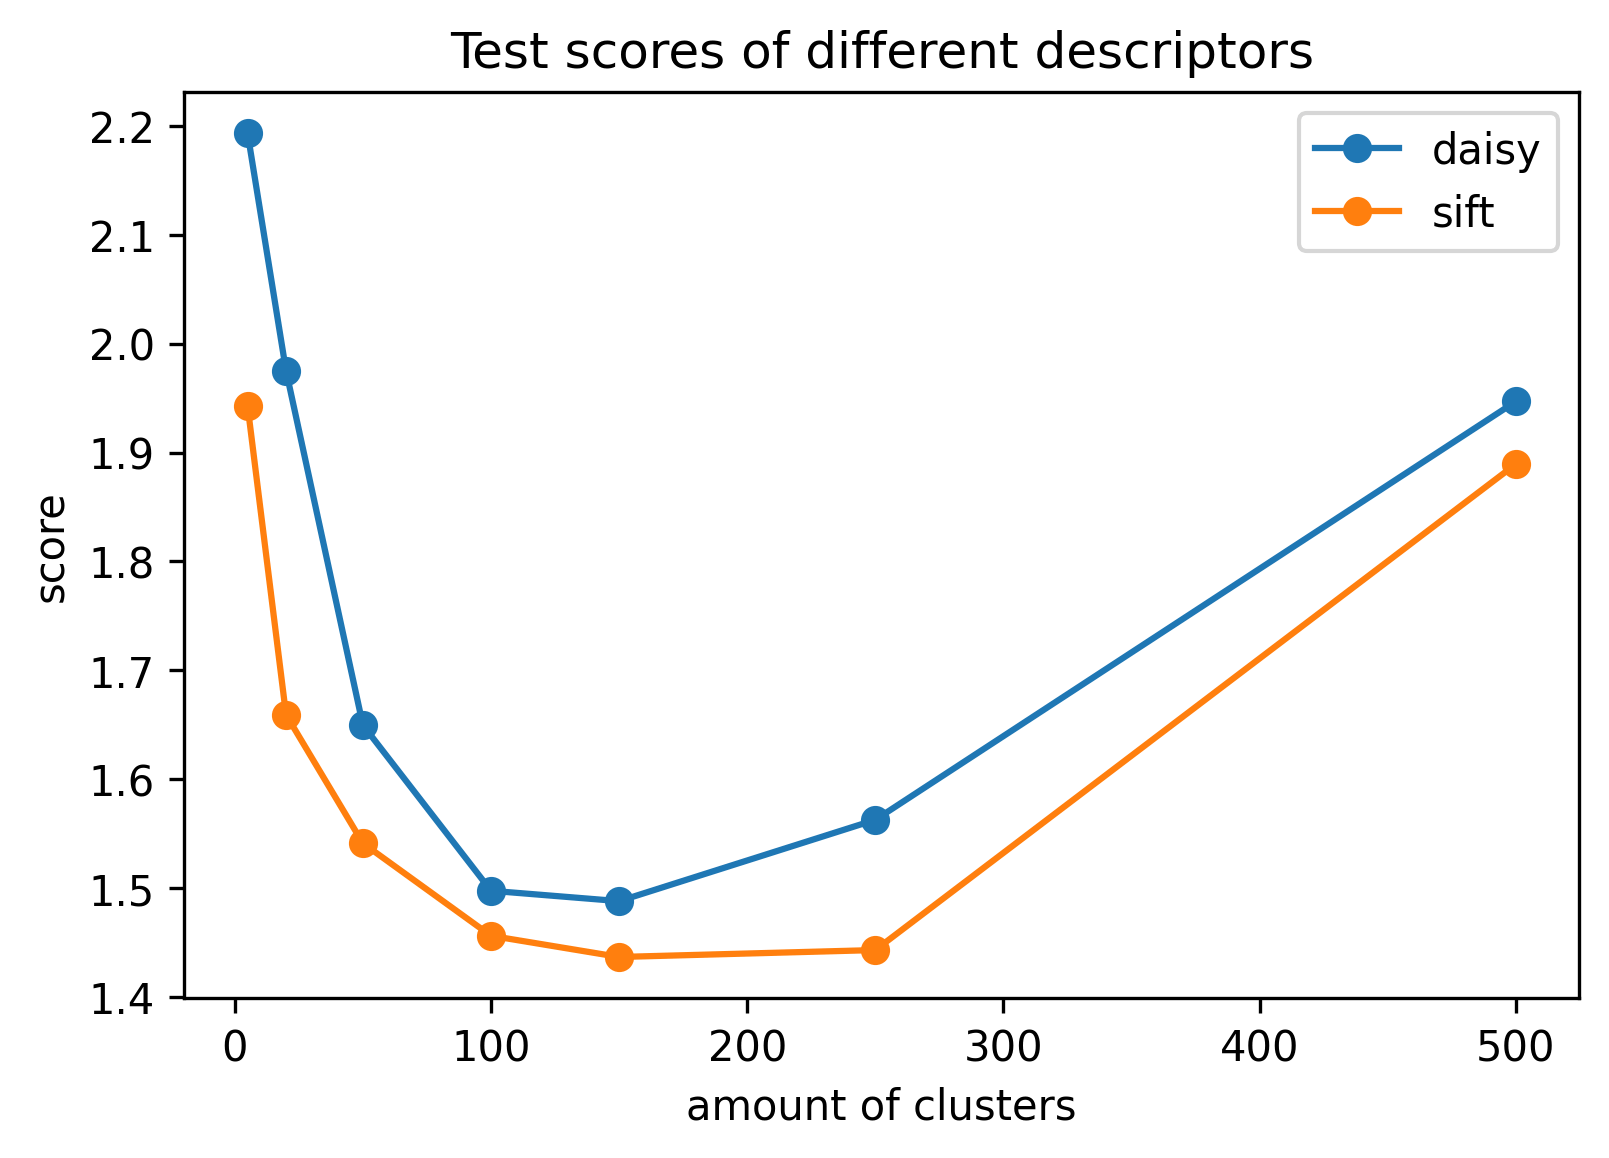
\includegraphics[width=\textwidth]{images/3/3_different_descriptors_test.png}}
        \captionsetup{width=0.9\linewidth}
        \captionsetup{justification=centering}
        \caption{Test scores.}
    \end{subfigure}
    \captionsetup{width=0.8\linewidth}
    \captionsetup{justification=centering}
    \caption{Averaged MCLL scores for optimal SVC model using different descriptors and clusters amounts over 3 trials. Lower score is better.}
    \label{fig:3-clusters}
\end{figure*}

\begin{wrapfigure}[13]{r}{0.6\textwidth}
    \centering
    \fbox{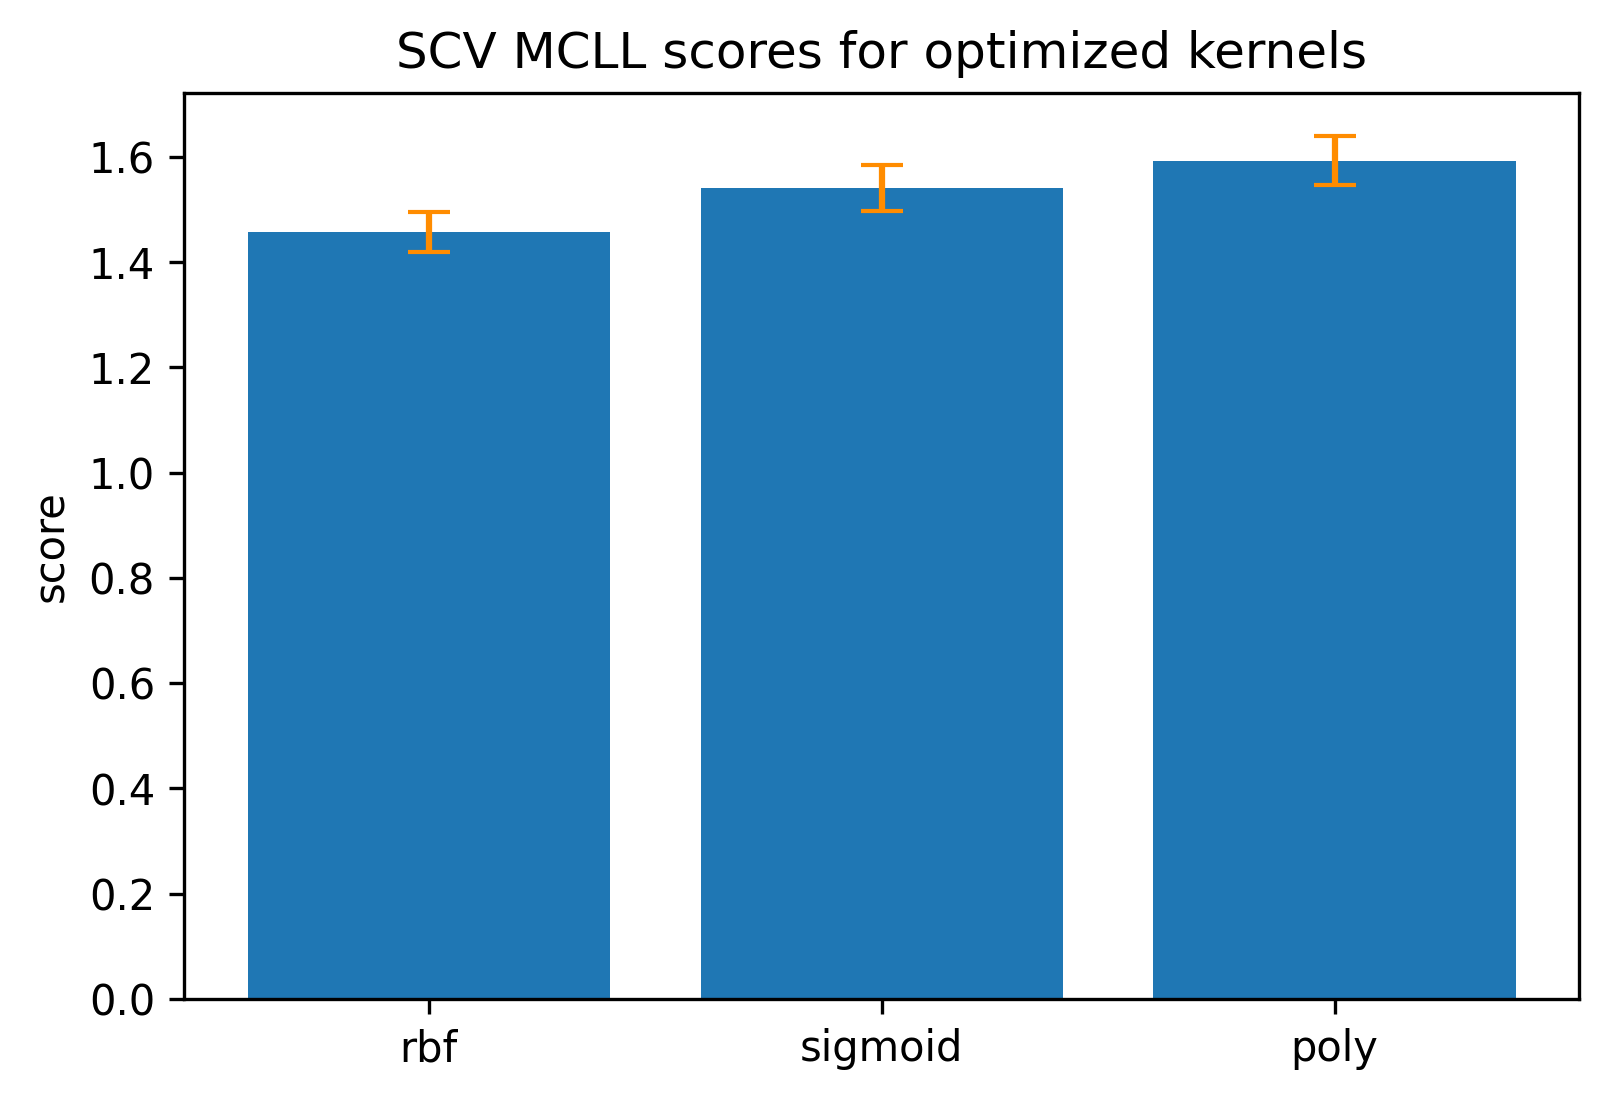
\includegraphics[width=0.75\linewidth]{images/3/SVC_optima_w_std.png}}
    \captionsetup{width=0.8\linewidth}
    \captionsetup{justification=centering}
    \caption{SCV MCLL score per kernel. \newline Lower score is better.}
    \label{fig:SVC_optima_w_std}
\end{wrapfigure}

A histogram showing the SCV MCLL score for each optimal kernel configuration together with the standard deviation is given in figure \ref{fig:SVC_optima_w_std}.
It is visible that the rbf kernel performed the best.
Thus, it was chosen to optimize this kernel further by doing another grid search that included more values around the found optima C and gamma.
The results from this further fine-tuning were negligible, C = 1.75 and gamma = 0.01 is used for the final model.

%------------------------------------

\section{The optimal settings for this model}
\label{section:svc_optimal}

The optimal settings and received score for the described model are:
\begin{itemize}
    \item Descriptor used: SIFT with 100 clusters
    \item Sample size for validation set: 15\%
    \item Class weight = balanced
    \item C =  1.75 | gamma = 0.01 | kernel = rbf | tol = 0.001
    \item MCLL score for validation set: ± 1.45 (balanced and unbalanced)
    \item SCV MCLL score: ± 1.48 (balanced and unbalanced)
    \item Score received on Kaggle: 1.55355 (non-balanced), 1.53626 (balanced)
\end{itemize}